\section{Organisation du travail}

%separation du travail, et choix de travaux en �quipe

\section{Les moyens techniques}

Afin de mener � bien notre projet, nous avons utilis�s un portail �volu� de
d�veloppement fournissant plusieurs outils : le portail berliOs.de \footnote{\url{http://www.berlios.de}}
\\ \newline
Pour am�liorer la communication avec notre client et notre responsable
p�dagogique, nous avons mis en place un wiki sur lequel on pouvait retrouver
toutes les principales informations relatives au projet.\\

\begin{figure}[h!t]
  \centering
  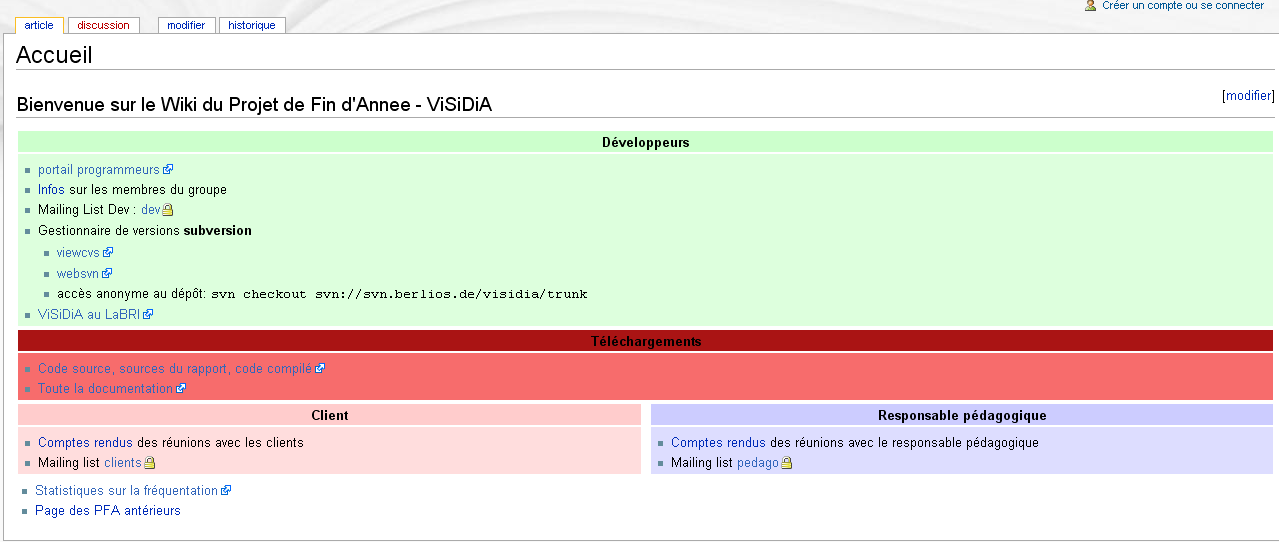
\includegraphics[width=10cm]{images/wiki.png}
  \caption{Le wiki du projet Visidia}
\end{figure}

Nous avons d�ploy�s plusieurs listes de diffusion pour faciliter la communication :
\begin{itemize}
  \item Une liste pour tous les d�veloppeurs
  \item Une liste de diffusion pour communiquer avec le client
  \item Une liste de diffusion pour communiquer avec le responsable p�dagogique \\
\end{itemize}

Nous avons utilis� �galement un gestionnaire de versions, Subversion
, qui nous permet de maintenir les sources de \visidia. 
Les clients ont �galement la possibilit� de
suivre l'avancement du projet et d'acc�der aux sources, gr�ce � deux
interfaces viewcvs  et websvn .  Il est
�galement possible de t�l�charger la derni�re version des sources du
projet:
\begin{verbatim}
svn checkout svn://svn.berlios.de/visidia/trunk
\end{verbatim}

\section{Avancement du projet}

%diagramme de gant a mettre la


